% Formação de imagem num espelho côncavo
% Feito para o ÉguaTeX (eguatex.com.br). Uso livre (CC0 1.0).
%
% Compile e pronto: sai só a figura, em PDF.
% Para pôr no seu trabalho, use o PDF com \includegraphics ou copie
% o bloco tikzpicture para dentro de uma figure.
%
% A posição e o tamanho da imagem saem da equação dos espelhos,
% 1/f = 1/p + 1/p', e do aumento A = -p'/p, com f = R/2.
% Use p maior que f para a imagem ser real e invertida.
% Como nos livros, os raios refletem na reta vertical do espelho
% (aproximação para raios perto do eixo).
\documentclass[tikz,border=4pt]{standalone}
\usepackage[T1]{fontenc}
\usepackage{lmodern}
\usetikzlibrary{patterns.meta}

\colorlet{corObj}{blue!70!black}
\colorlet{corImg}{red!75!black}
\colorlet{corRaio}{orange!85!black}

\begin{document}
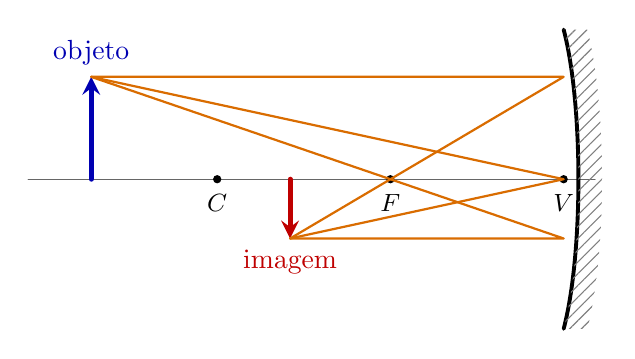
\begin{tikzpicture}[line cap=round, line join=round, >=stealth,
  raio/.style={line width=0.8pt, corRaio},
  seta/.style={->, line width=1.8pt}]

% Mude estes números e o desenho e os rótulos acompanham.
\def\f{2.2}   % distância focal, em cm (o centro C fica em 2f)
\def\p{6}     % distância do objeto até o espelho, em cm (maior que f)
\def\h{1.3}   % altura do objeto, em cm

\pgfmathsetmacro{\q}{1/(1/\f-1/\p)}   % distância da imagem
\pgfmathsetmacro{\hi}{-\h*\q/\p}      % altura da imagem (negativa: invertida)
\pgfmathsetmacro{\L}{max(\p,\q,2*\f)+0.8}
\pgfmathsetmacro{\H}{max(\h,-\hi)+0.6}

% eixo e espelho (o espelho fica em x = 0, os objetos à esquerda)
\draw[black!60] (-\L,0) -- (0.4,0);
\draw[line width=1.4pt] (0,\H) .. controls (0.25,{\H/2}) and (0.25,{-\H/2}) .. (0,-\H);
\fill[pattern={Lines[angle=45, distance=3pt, line width=0.4pt]}, pattern color=black!50]
  (0,\H) .. controls (0.25,{\H/2}) and (0.25,{-\H/2}) .. (0,-\H) -- (0.3,-\H)
  .. controls (0.55,{-\H/2}) and (0.55,{\H/2}) .. (0.3,\H) -- cycle;
\foreach \x/\n in {-\f/F, {-2*\f}/C, 0/V} {
  \fill (\x,0) circle[radius=1.5pt];
  \node[below=2pt, font=\small] at (\x,0) {$\n$};
}

% objeto e imagem
\draw[seta, corObj] (-\p,0) -- (-\p,\h) node[above] {objeto};
\draw[seta, corImg] (-\q,0) -- (-\q,\hi) node[below] {imagem};

% raios notáveis
% 1: paralelo ao eixo, reflete passando pelo foco F
\draw[raio] (-\p,\h) -- (0,\h) -- (-\q,\hi);
% 2: passa pelo foco F, reflete paralelo ao eixo
\draw[raio] (-\p,\h) -- (0,\hi) -- (-\q,\hi);
% 3: chega ao vértice V e reflete simétrico ao eixo
\draw[raio] (-\p,\h) -- (0,0) -- (-\q,\hi);
\end{tikzpicture}
\end{document}
